\documentclass[12pt,a4j,fleqn]{jsarticle}
\usepackage{geometry}
\usepackage{amsmath}
\usepackage{amssymb}
\usepackage{txfonts}
\usepackage{bm}
\usepackage[dvipdfmx]{graphicx}
\usepackage{booktabs}
\geometry{top=20truemm,bottom=15truemm,left=25truemm,right=10truemm}
\linespread{0.97}  % 1 ページ 40 行
\renewcommand{\figurename}{Fig.~}
\renewcommand{\tablename}{Table~}
\setlength{\mathindent}{2em}
\pagestyle{empty}
\begin{document}
\begin{center}
\textsf{\textgt{\Large Study on higher order of basis functions for S-version Isogeometric Analysis Method}}
\end{center}
\vspace{\baselineskip}
\begin{flushleft}
[Okada Group]
\end{flushleft}
\vspace{-2\baselineskip}
\begin{flushright}
7518074 Yuhi TSUCHIYAMA
\end{flushright}
In Finite Element Method (FEM), it is estimated that
the design of the analytical model accounts for about $80\ \%$ of the total analysis.
%
In recent years, Meshfree method have been studied in order to shorten the generation of analytical models.
%
One of them is Isogeometric Analysis (IGA),
which uses Non-Uniform Rational B-Spline (NURBS),
a geometric representation of CAD,
as basis functions.
%
In addition, the S-version Finite Element Method (S-FEM),
which is a multi-scale analysis that enables flexible modeling and high accuracy of FEM analysis,
has been proposed to be applied to IGA analysis, S-version Isogeometric Analysis Method (S-IGA).
%
In this study, examples of IGA analysis and S-IGA analysis
with higher order of basis functions are presented to verify the accuracy of the analysis.
%
In the IGA analysis, as shown in Figure \ref{fig:1},
the third-order basis functions were more accurate than the second-order basis functions for the same degrees of freedom.
%
In the S-IGA analysis, the highest accuracy was obtained when the order of basis functions was set to the third-order for both the Global and Local patches.
%
As shown in Figure \ref{fig:2} and Figure \ref{fig:3}, the distribution of results was smoother when the third-order basis functions were used.
%
It was also confirmed that setting the ratio of the overall size of the Local patch to the element size of the Global patch
between 2.5 and 4 times prevented the phenomenon of reduced analysis accuracy.

\begin{figure}[htbp]
  \centering
  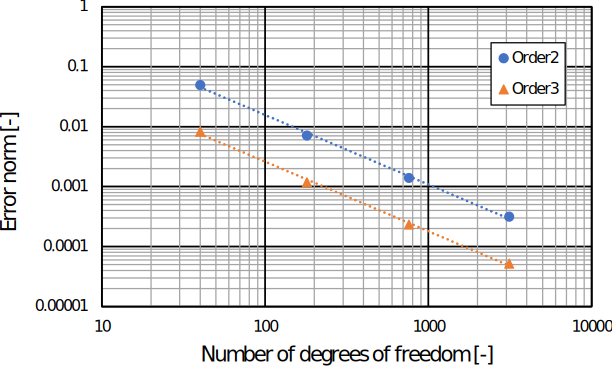
\includegraphics[keepaspectratio, scale = 0.7]
  {fig/ER01-crop.pdf}
  \caption{Error norm of $\sigma_{rr}$ in the IGA analysis}
  \label{fig:1}
\end{figure}

\clearpage

\begin{figure}[hbtp]
  \begin{tabular}{cc}
    \begin{minipage}[t]{0.45\hsize}
      \centering
      \includegraphics[keepaspectratio, scale=0.3]
      {fig/2.png}
      \caption{Stress in $y$ direction on Local patch in the S-IGA analysis (second-order, Global patch $30\times 30$, Local patch $20\times 20$)}
      \label{fig:2}
    \end{minipage} &
    \begin{minipage}[t]{0.45\hsize}
      \centering
      \includegraphics[keepaspectratio, scale=0.3]
      {fig/3.png}
      \caption{Stress in $y$ direction on Local patch in the S-IGA analysis (third-order, Global patch $30\times 30$, Local patch $20\times 20$)}
      \label{fig:3}
    \end{minipage}
  \end{tabular}
\end{figure}
\end{document}
